% !TeX root = /../Report.tex

\chapter{Chosen Master Devices and Characteristics}\label{chosenDevices}
Every device was chosen to control independently each one of the catheter's DOF as shown in figure~\ref{img:dofi}. In this section the mechanics, electronics and functioning of every input device is explained. After, a comparison between all device's characteristics, advantages and disadvantages is made.

\begin{figure}[ht]
   \centering
   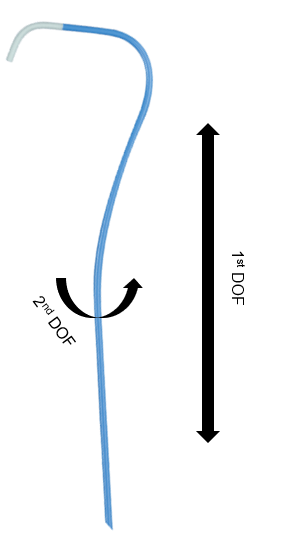
\includegraphics[width=0.4\textwidth]{img/Dof.PNG}
   \caption{TAVI catheter degrees of freedom}
   \label{img:dofi}
\end{figure}

\section{Keyboard}\label{sec:keyboard}
The keyboard device intends to represent any other device only controlled by on-off buttons, working in a digital configuration. For this experiment a numerical keypad was used (figure~\ref{img:keyboardimg}).\\

The control of the catheter was performed with the arrow key, with the UP and Down arrow key the controlling the 1st DOF of the catheter. The 2nd DOF was controlled with the RIGHT and LEFT arrow keys.\\

Both types of movements are mapped to the simulated catheter with a PressedTime-Velocity mapping. For information about the mapping refer to section~\ref{sec:mapping}.\\

\begin{figure}[ht]
   \centering
   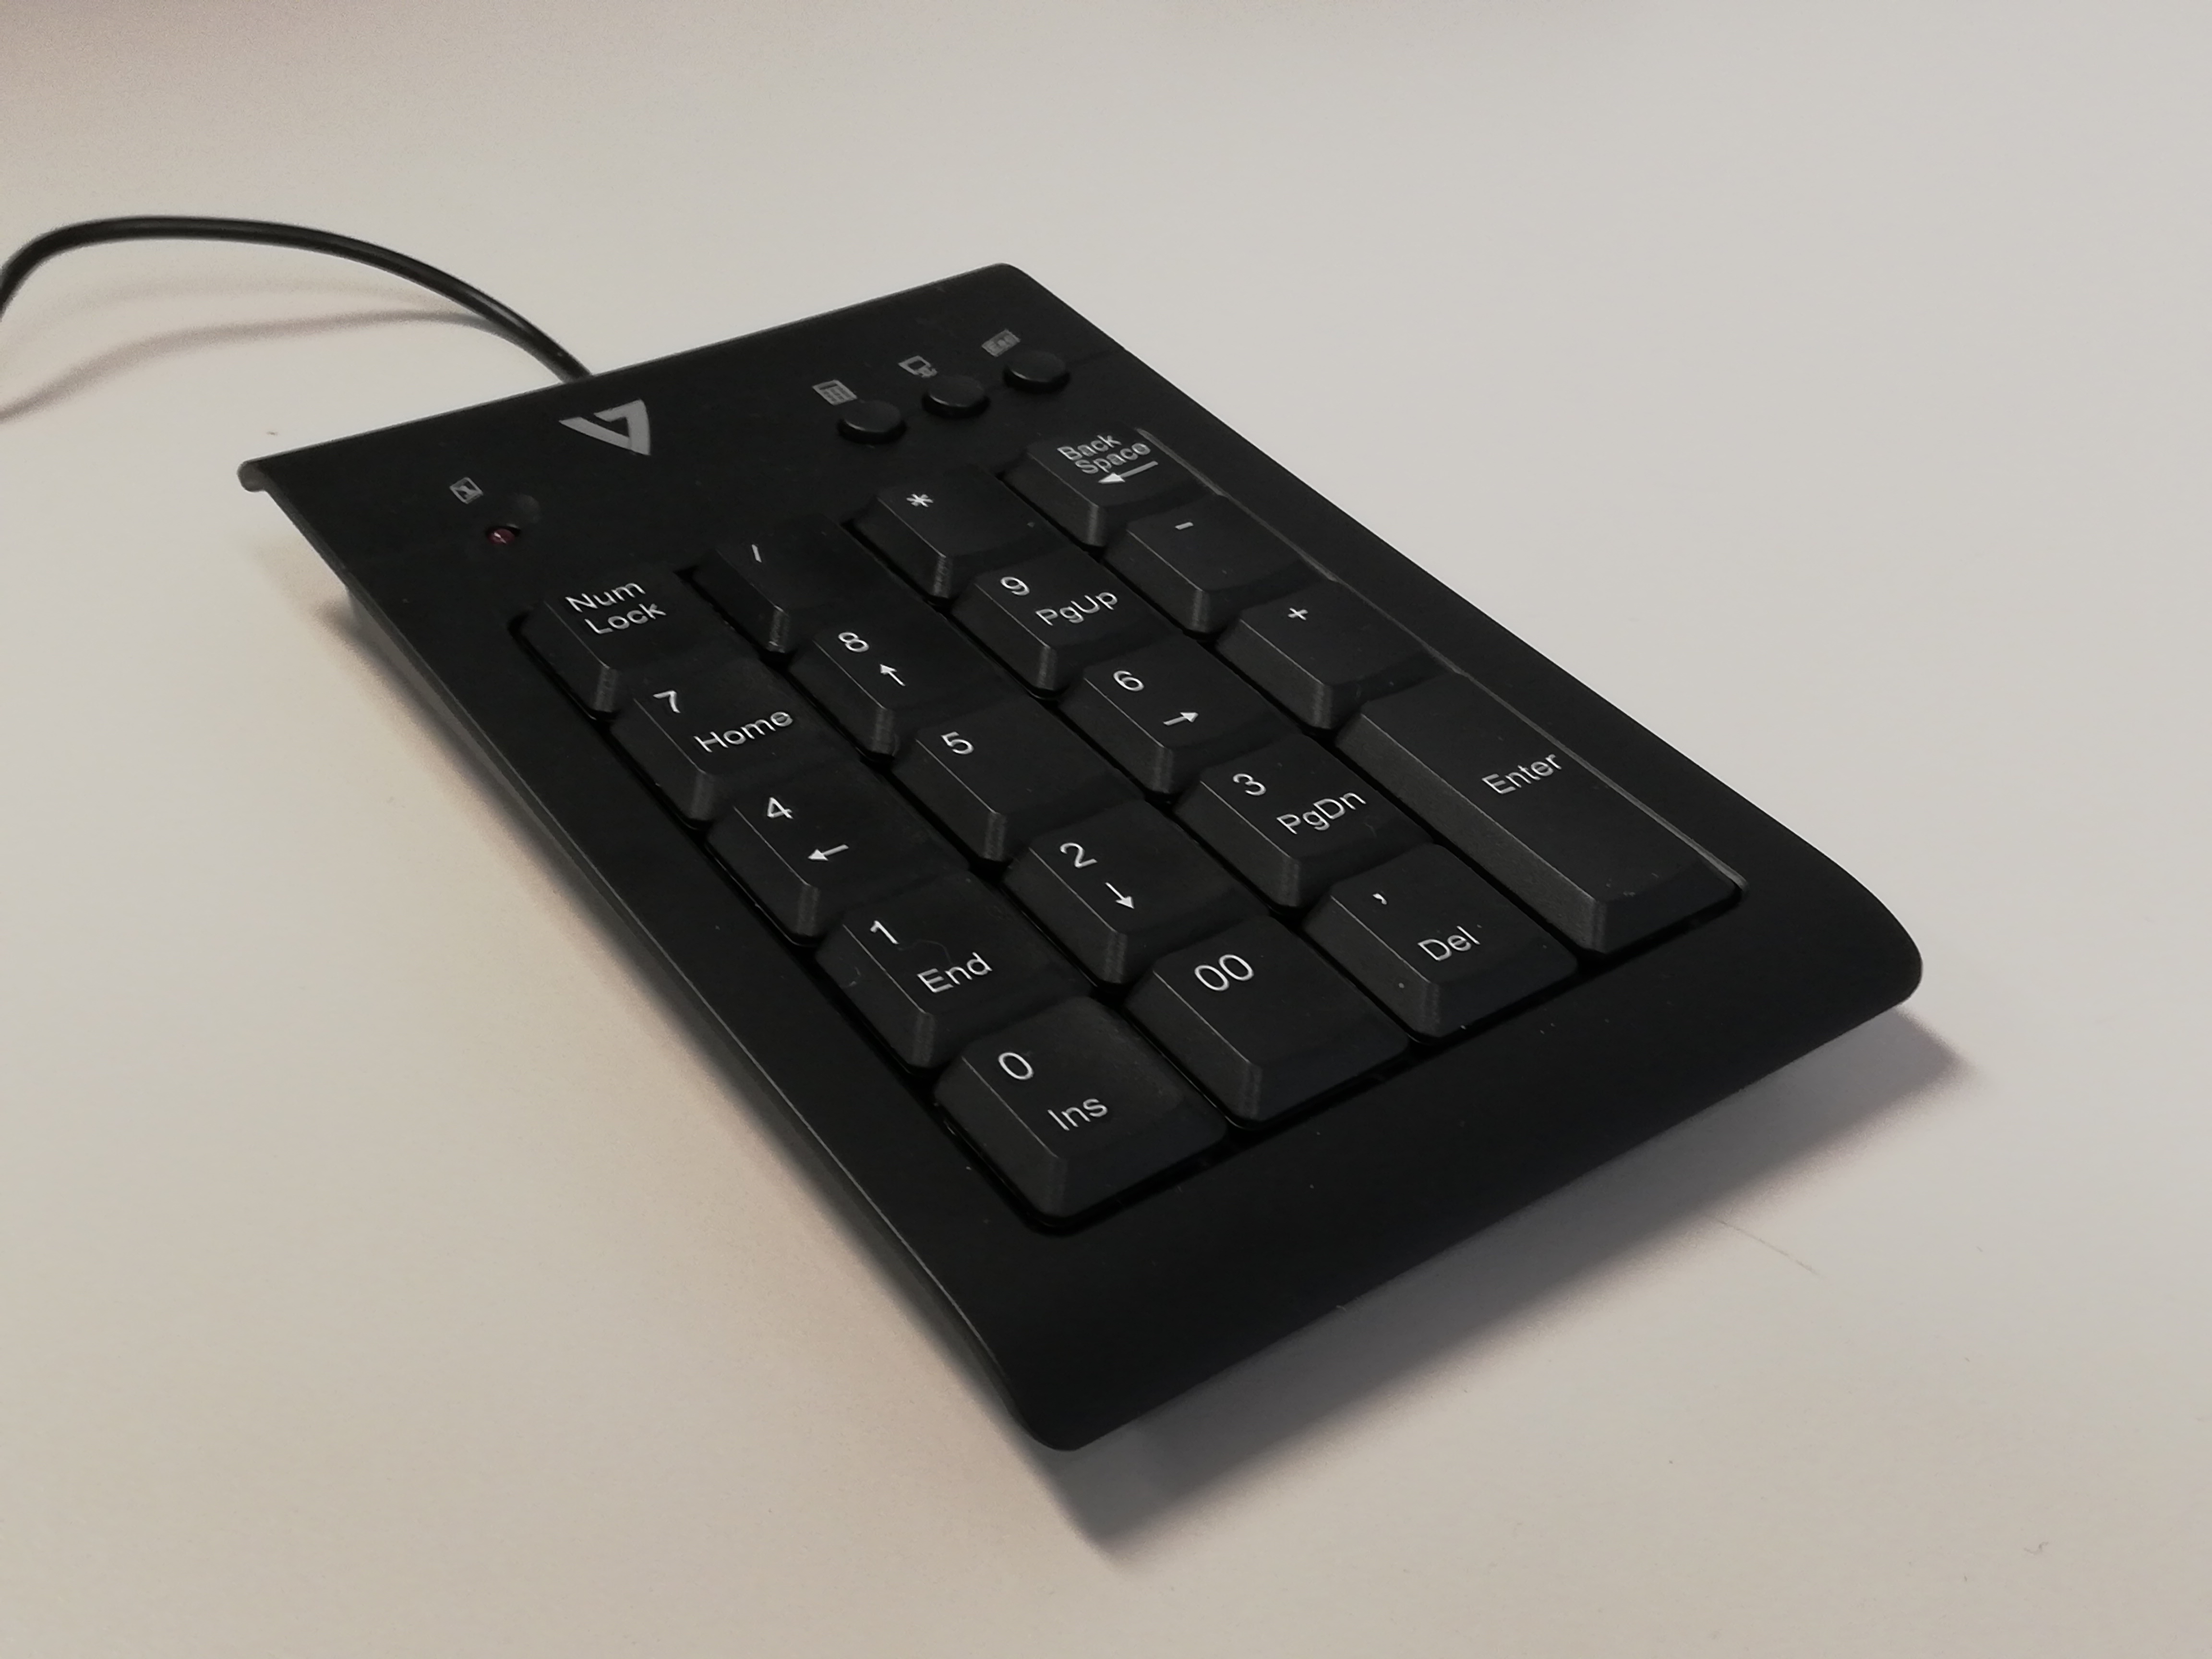
\includegraphics[width=0.7\textwidth]{img/keyboard.jpg}
   \caption{Keypad model V7-KP1019-USB-4EB with USB connection}
   \label{img:keyboardimg}
\end{figure}

\section{Remote}\label{sec:remote}
The Remote device is a combination of on-off buttons and a semi-analogical sensor (figure~\ref{img:remotecad} and~\ref{img:remotenorm}). The shell of the device was 3D printed in ABS. It is also equipped with two push buttons, and a continuous 360 degrees rolling disk.\\

The 1st DOF of the catheter is controlled using the two push buttons in a digital configuration. Movements in this DOF are mapped to the simulated catheter with a PressedTime-Velocity mapping.\\

The 2nd DOF is controlled by a non-contacting rotatory position sensor attached to the rolling disk, which gives a semi-analogical reading with a 12 BIT resolution per 360 degrees. It is important to notice that the experiment setup as can be seen in section~\ref{sec:arddevinter} uses an Arduino with a 10BIT ADC channel, which trims the initial sensor's 12BIT resolution. Movements in this DOF are mapped using a Velocity-Velocity mapping.\\

For information about the mapping refer to section~\ref{sec:mapping}.\\

\begin{figure}[ht]
   \centering
   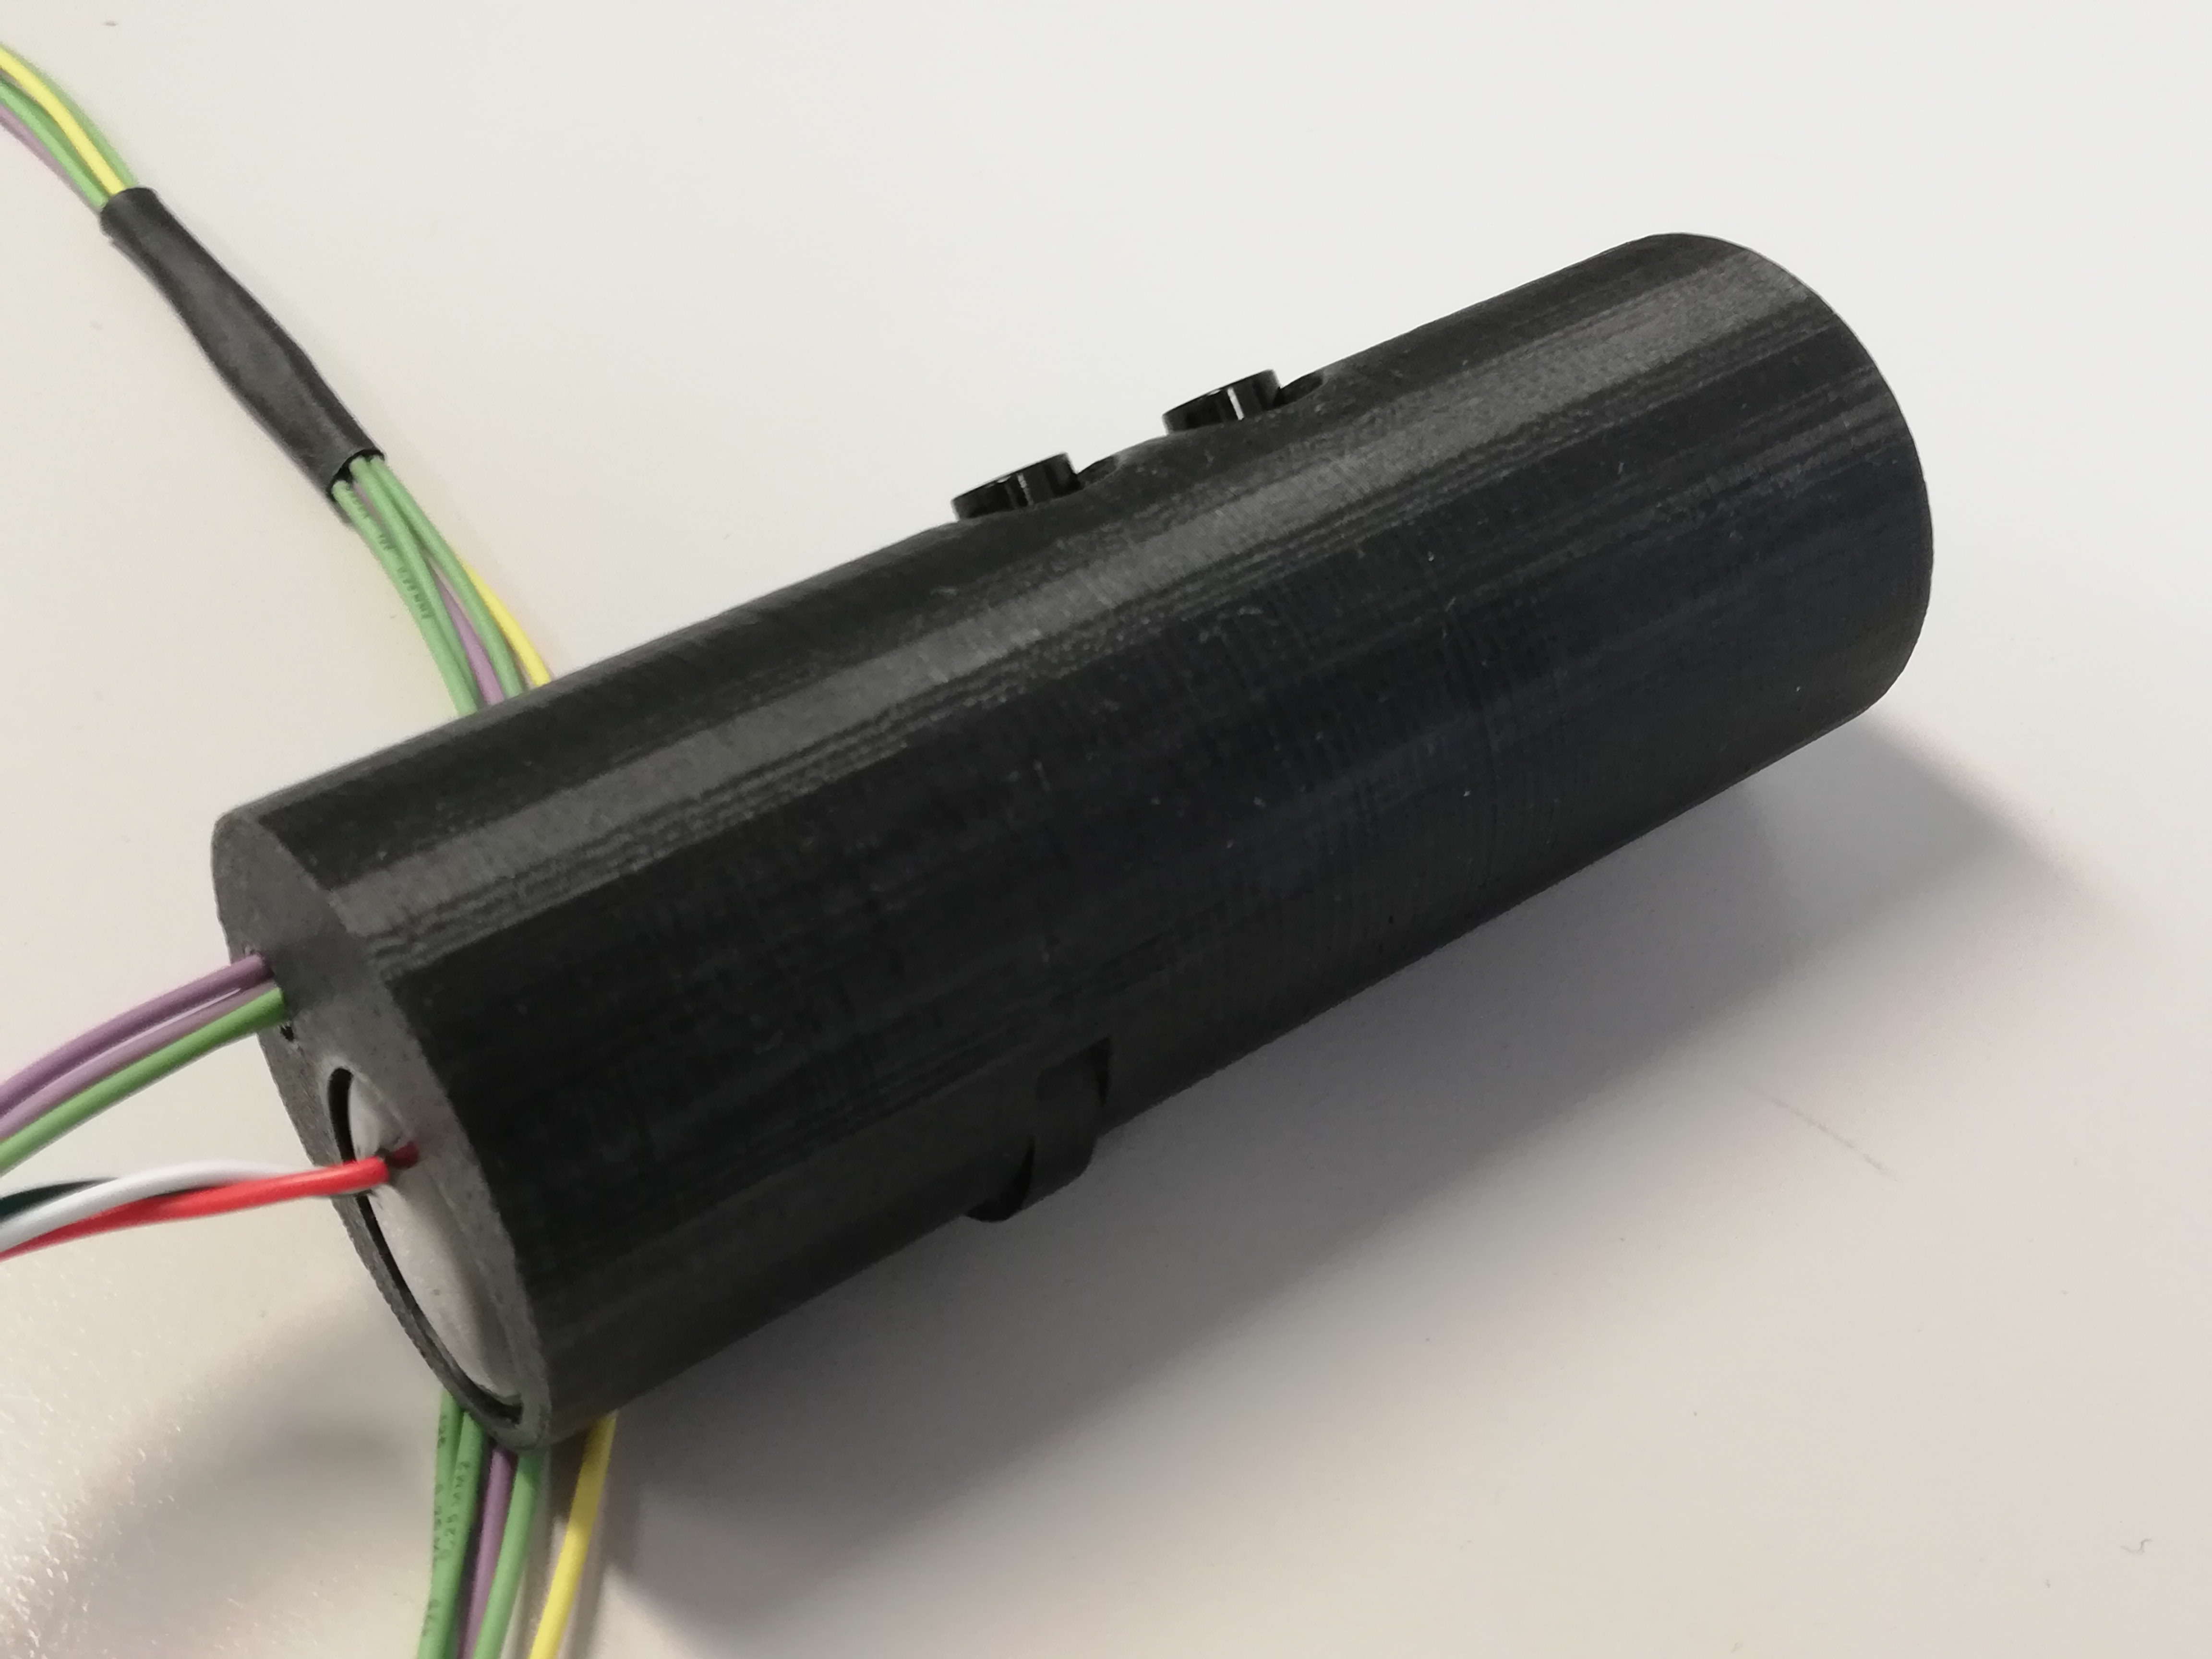
\includegraphics[width=0.7\linewidth]{img/remote.jpg}
   \caption{Remote device used for the experiments}
   \label{img:remotenorm}
\end{figure}

\begin{figure}[ht]
   \centering
   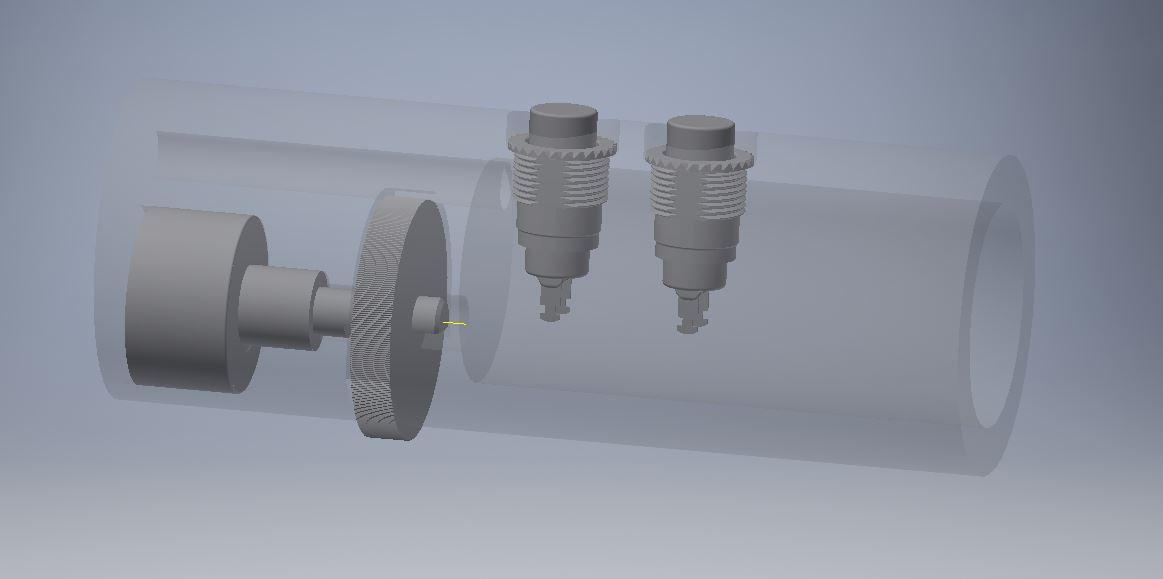
\includegraphics[width=0.7\linewidth]{img/remotecad.jpg}
   \caption{CAD design of the remote device (push buttons C\&K 8532T1ZBE2) (Rotatory sensor CTS 285CCDFSAAB4C1)}
   \label{img:remotecad}
\end{figure}

\section{Joystick}\label{sec:joystick}

The Joystick device is implemented with fully analogical sensors (figure~\ref{img:joystickimg}). Originally the Joystick had 3 DOF available, plus a push button on the top. The roll DOF and the button are not connected at all. Thus, performing any movement on them will not make any difference in the outputs.\\

The 1st DOF of the catheter is controlled by a regular 5Kohm potentiometer, mapped on the pitch movement of the joystick. The movements in this DOF are translated to the simulation catheter with a Distance-Velocity mapping.\\

The 2nd DOF is also controlled by regular 5Kohm potentiometer mapped to the yaw movement of the joystick.\\

The two DOF used, pitch and yaw, are limited on their angle and brought back automatically to initial position by springs once any force is applied. The movements in both DOF are translated into the simulated catheter with a Position-Velocity mapping. For information about the mapping refer to section~\ref{sec:mapping}. \\

The potentiometers have essentially infinite resolution, only trimmed by the Arduino's ADC channel (See section~\ref{sec:arddevinter} for experiment setup) used to read out the sensors.\\

\begin{figure}[ht]
   \centering
   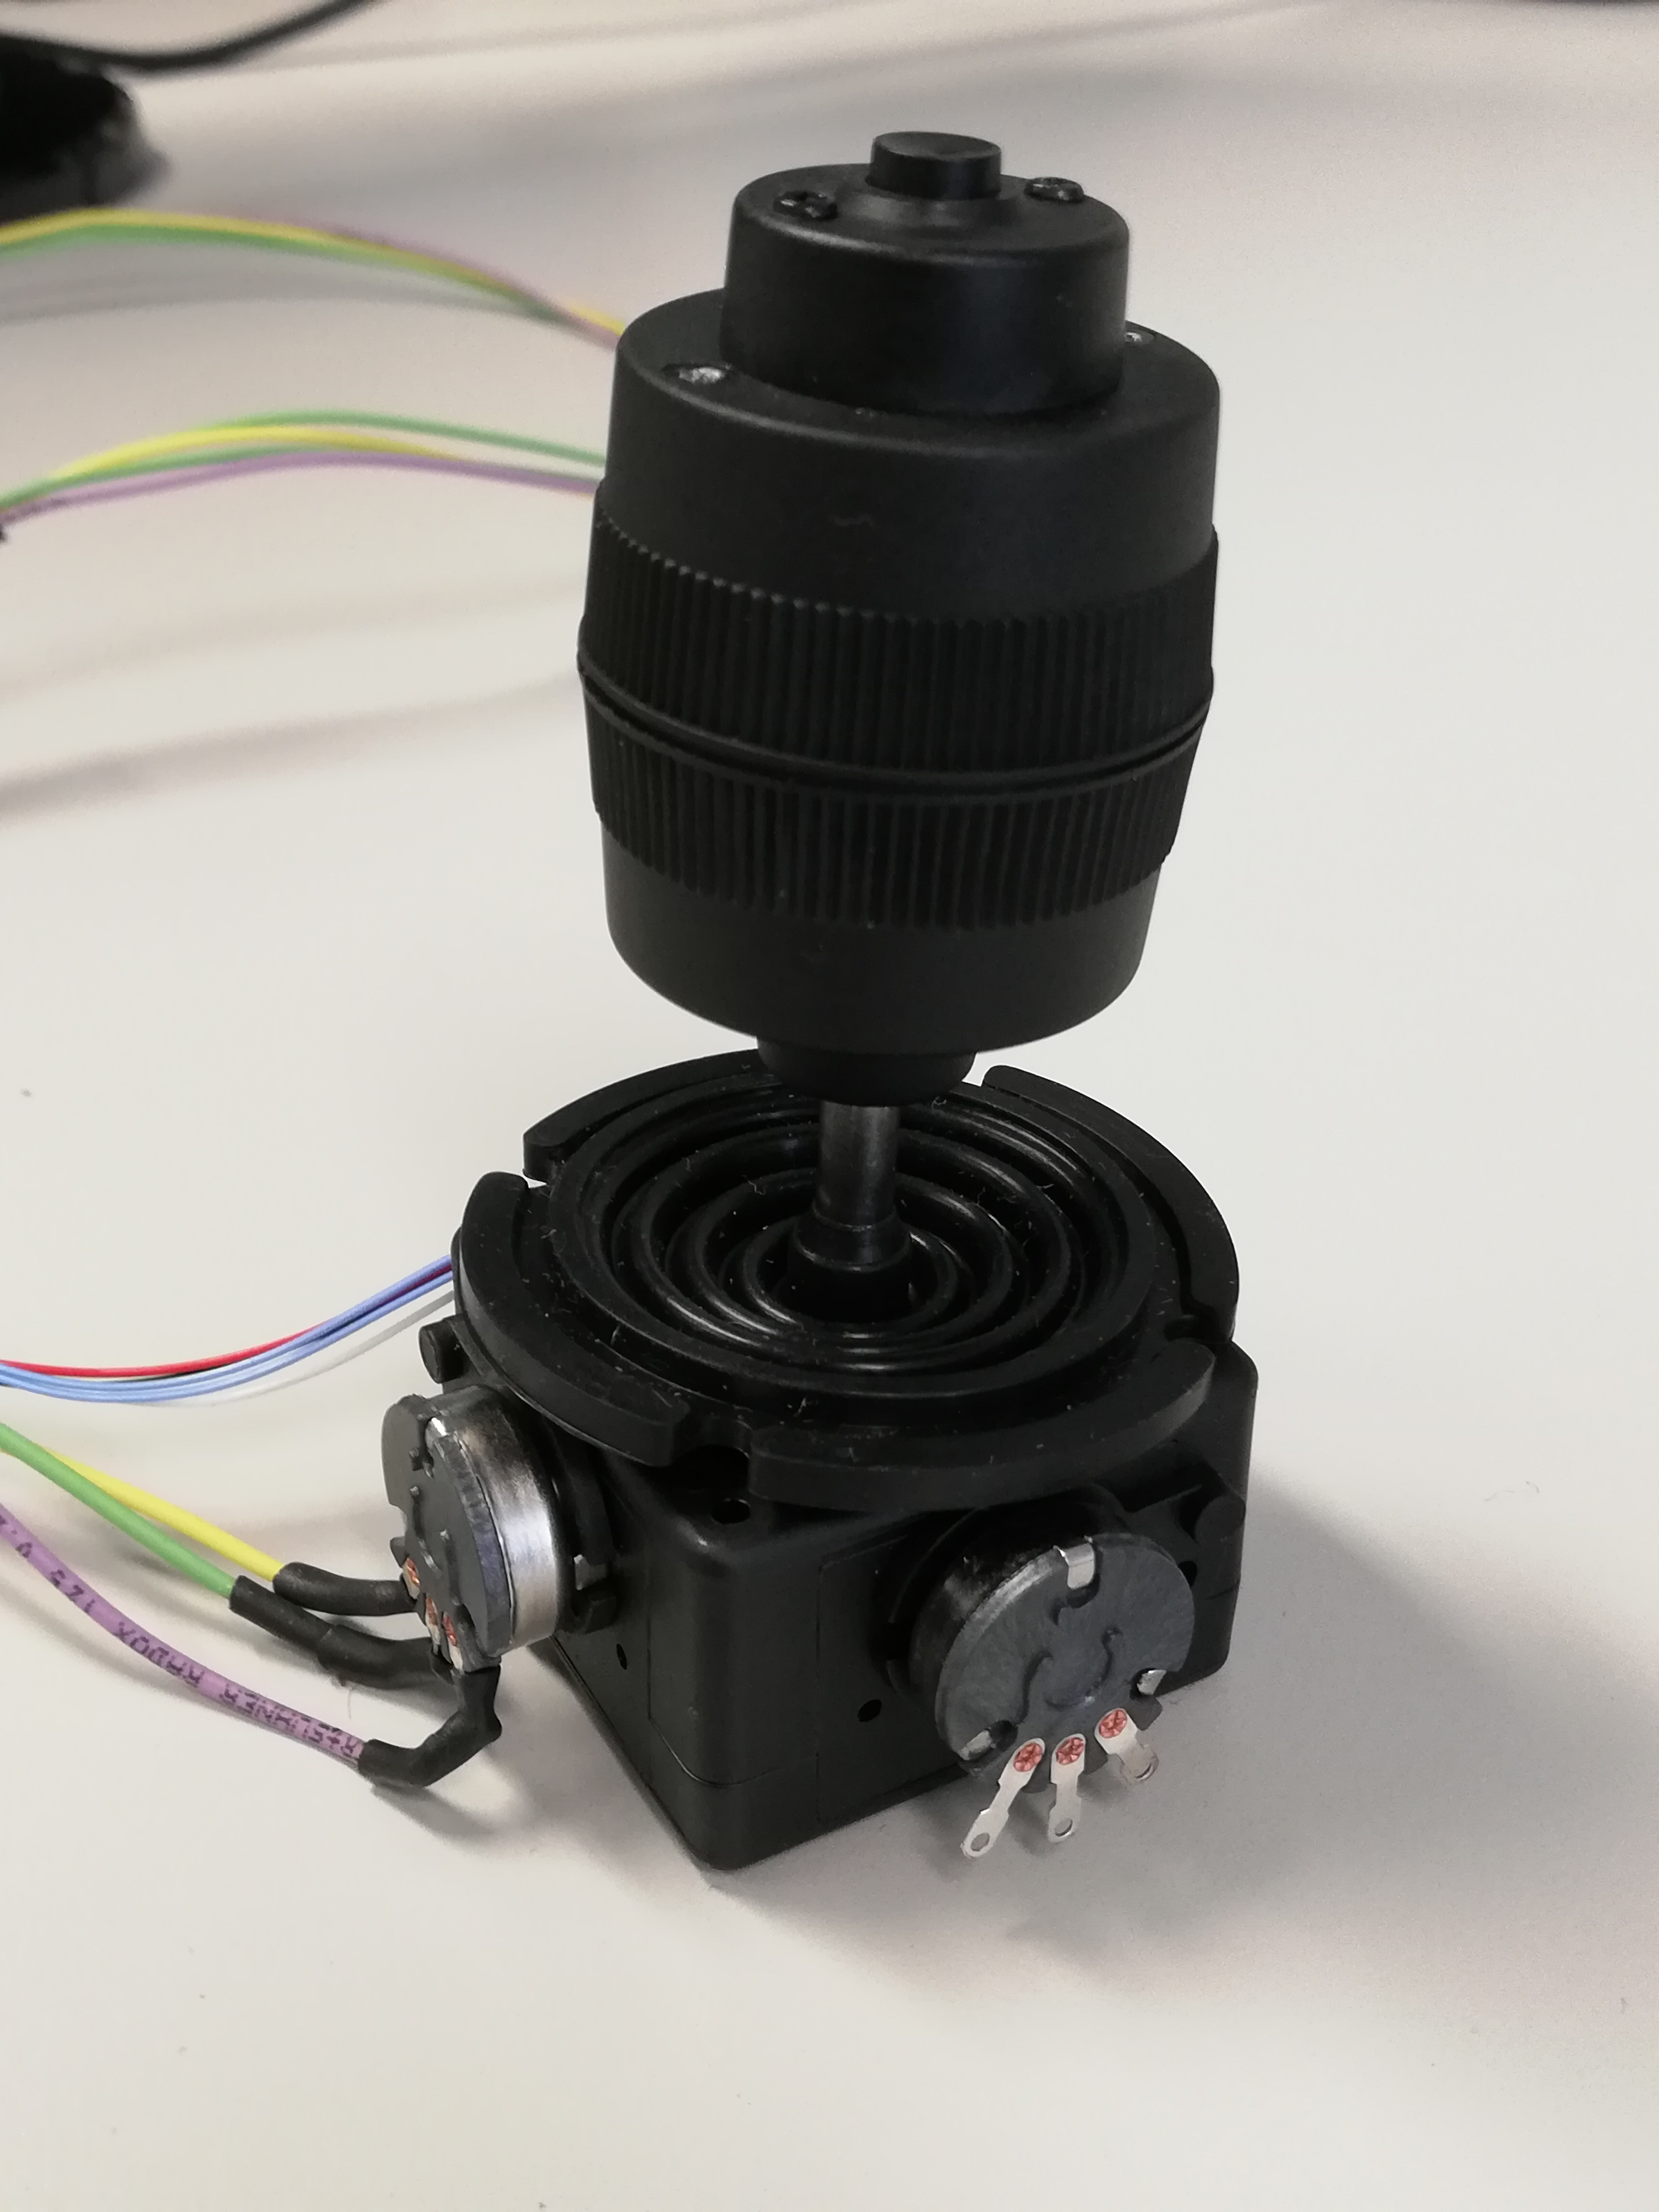
\includegraphics[width=0.6\linewidth]{img/joystick.jpg}
   \caption{Joystick used for the experiments}
   \label{img:joystickimg}
\end{figure}

\section{CatheterLike}\label{sec:catheterlike}
The CatheterLike device is a combination of an analogic sensor and a semi-analogic sensor, figure~\ref{img:catheterimg} and~\ref{img:cathetercad}. The shell of the device was 3D printed in ABS. The device has a handle on the outside that can be pushed and pulled axially coming back automatically to resting position (activated by springs), and can also be rotated over its own axis continuously 360 degrees.\\

The 1st DOF of the catheter is controlled by a 10Kohm and 30mm slide potentiometer. Activated by the push and pull movement on the device, it is mapped to the simulated catheter with a Position-velocity mapping.\\

The 2nd DOF is activated by the rotation of the device, mapped Velocity-Velocity to the simulated catheter and controlled by a non-contacting rotatory position sensor, which gives a semi-analogical reading with a 12 BIT resolution per 360 degrees. It is important to notice that the experiment setup as can be seen in section~\ref{sec:arddevinter} uses an Arduino with a 10BIT ADC channel, which trims the initial sensor's 12BIT resolution.\\

For information about the mapping refer to section~\ref{sec:mapping}.\\

\begin{figure}[ht]
   \centering
   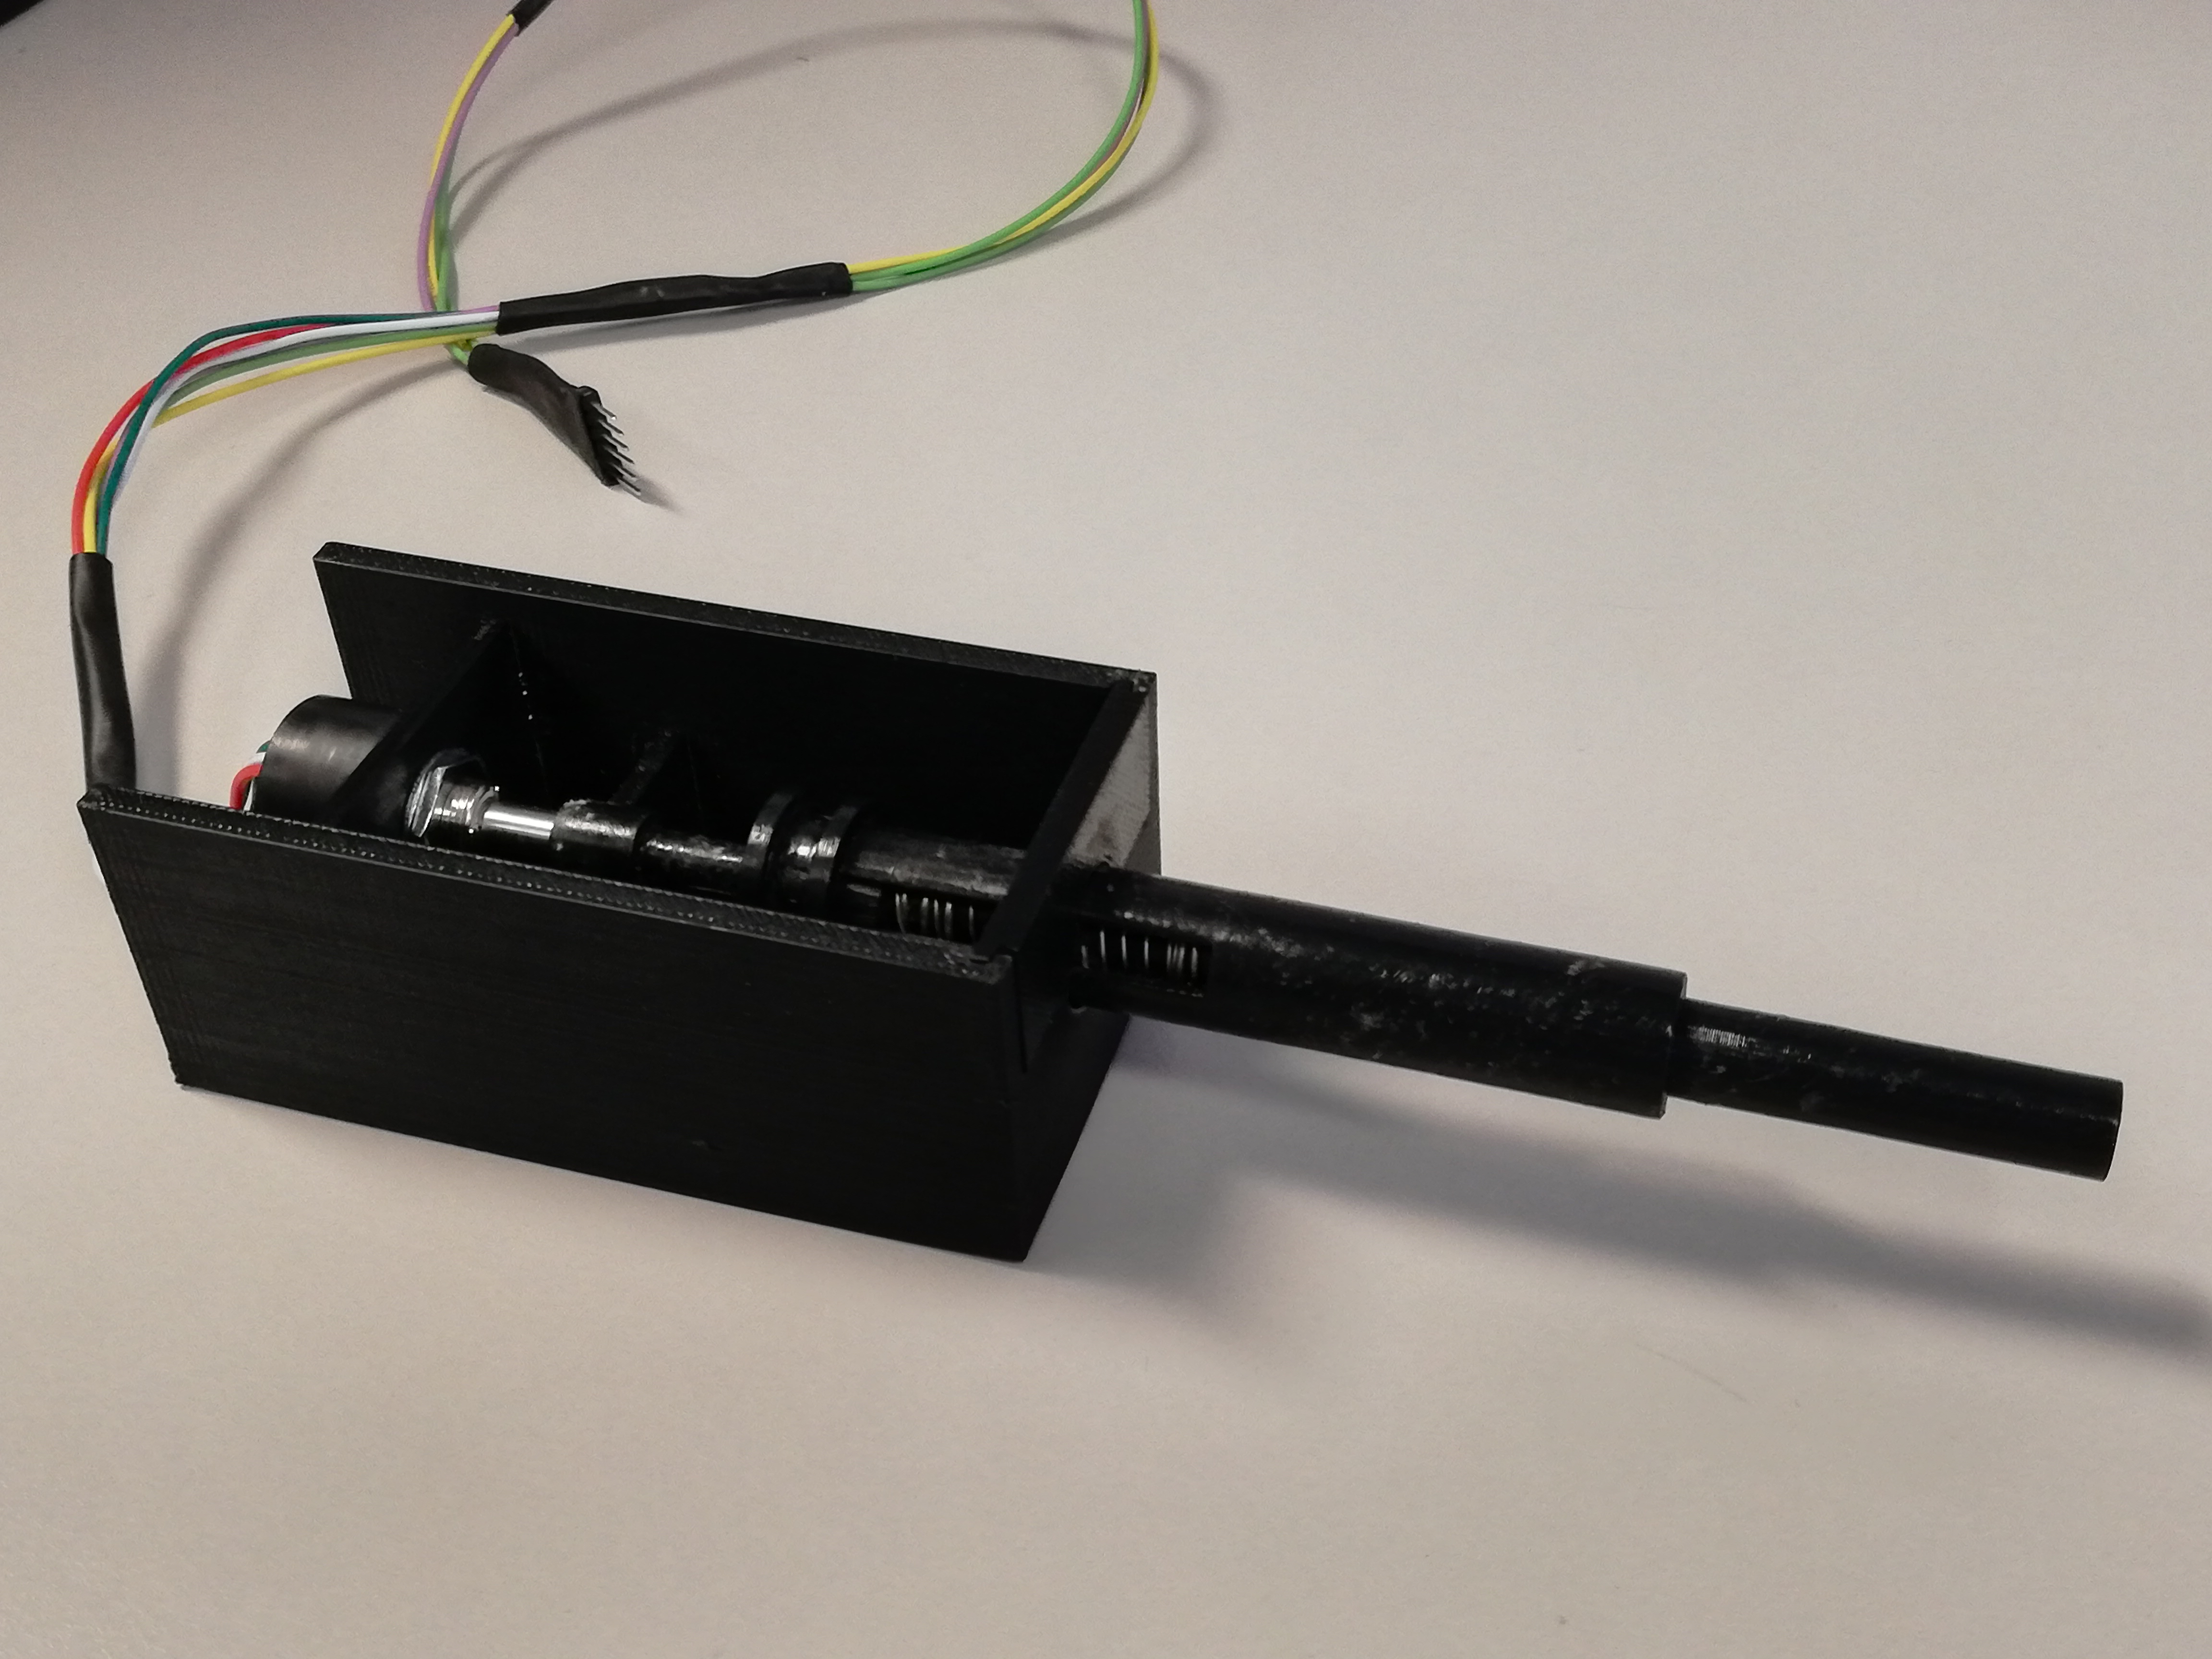
\includegraphics[width=0.7\linewidth]{img/catheter.jpg}
   \caption{CatheterLike device used for the experiment}
   \label{img:catheterimg}
\end{figure}

\begin{figure}[ht]
   \centering
   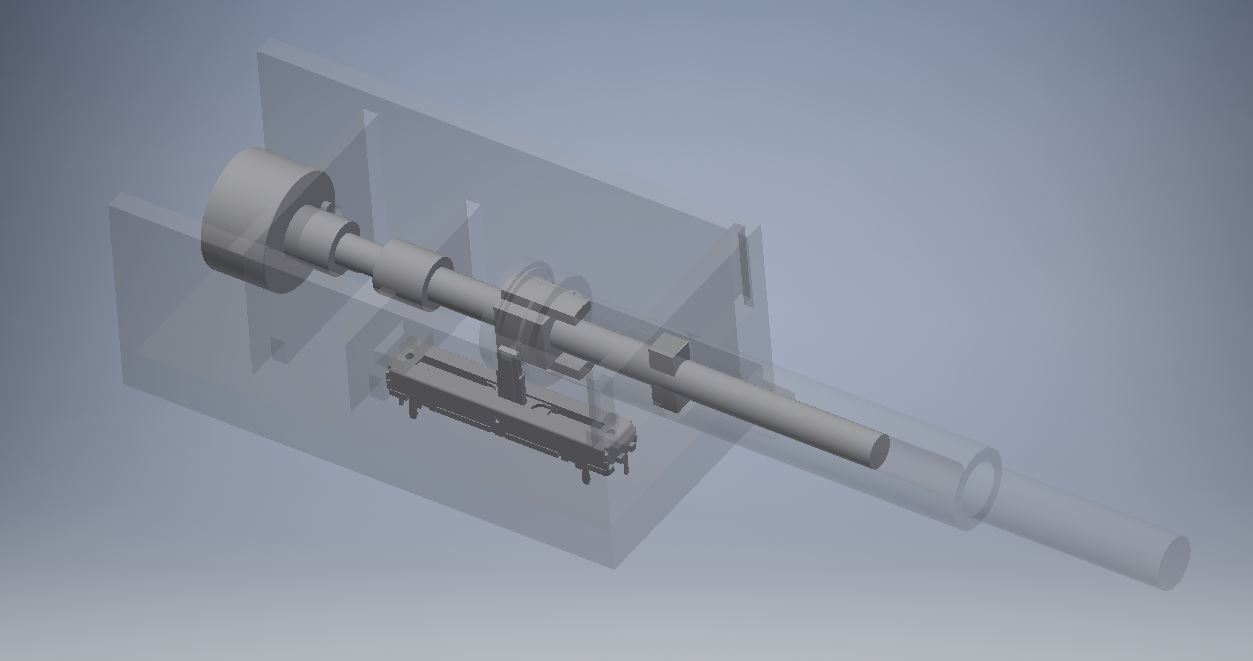
\includegraphics[width=0.7\linewidth]{img/cathetercad.jpg}
   \caption{CAD design of the catheter like design (Slide Pot PTA3043-2210CIB103) (Rotatory sensor CTS 285CCDFSAAB4C1)}
   \label{img:cathetercad}
\end{figure}

\section{Mapping Types, Advantages and Disadvantages}\label{sec:mapping}
Every device with its different type of sensor is better adapted for a specific mapping. This means, how specific movements in each one of the devices, in each one of its degrees of freedom, translates to movements on the simulation catheter.\\

The \textbf{PressedTime-Velocity} mapping was created to mitigate the clear disadvantage devices with on-off buttons have against analogical/semi-analogical ones. This disadvantage is due to the fact that on-off devices have always the same speed applied over the catheter. If that speed is too high, it is not possible to apply small movement. On the other hand, if it is too low, it would take too much time to perform long movements. On the contrary, analogical sensor devices have a wide range resolution from where low and high speeds can be applied in the same configuration.\\

This mapping consists in incrementing the output velocity linearly with a defined slope in relation with the time the button was pressed, starting from an initial offset, eq~\ref{eq:1steq}.\\

\begin{equation}
   \scalebox{1.2}{$outputVel=constant+(constant*pressedTime)$}
   \centering
   \label{eq:1steq}
\end{equation}

The \textbf{Position-Velocity} mapping is used in devices with analogical sensors, mapping linearly with a defined slope the position of the sensors to the velocity of the output catheters, eq~\ref{eq:2ndeq}.\\

\begin{equation}
   \scalebox{1.2}{$outputVel=sign(position)*max(0,abs(position-threshold))*constant$}
   \centering
   \label{eq:2ndeq}
\end{equation}

The threshold variable is meant to create a dead zone around the resting point of the device, given that the mechanism that automatically returns the device to the resting point is never perfect and it is also important to avoid accidental activation movements on the simulated catheter.\\

The \textbf{Velocity-Velocity} mapping is used for the semi-analogical rotatory sensors, which are able to rotate continuously 360 degrees (multi turn). This method maps the velocity of the device to the velocity of the simulated catheter, multiplied by a constant, eq~\ref{eq:3rdeq}.\\

\begin{equation}
   \scalebox{1.2}{$outputVel=\frac{deviceCount(k)-deviceCount(k-1)}{Ts}*constant$}
   \centering
   \label{eq:3rdeq}
\end{equation}

Using these type of sensors simplifies the mechanics of the device but adds an additional challenge when getting the information from the Arduino to Matlab (See Experiment Environment section~\ref{sec:matardinter} for setup). This happens because the sample rate the Arduino board has to sample the device is much faster than the sample rate from Matlab to the Arduino, which makes the simulation take noisy data and the behavior of the simulation catheter look highly erratic. In order to overcome this and make the user experience smoother, the Arduino sample rate has to match with the Matlab simulation sample rate (Being Ts on eq~\ref{eq:3rdeq} now the Matlab sample rate), making Arduino to implicitly take the average of all the movements between samples.\\

All the advantages and disadvantages are presented in figure~\ref{img:adtable}.\\

\begin{figure}[ht]
   \centering
   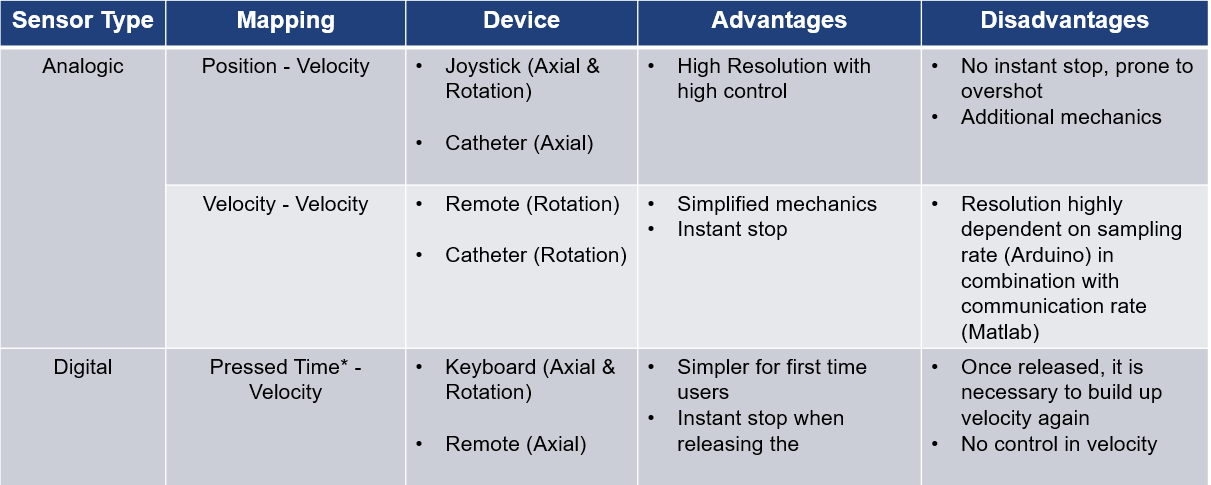
\includegraphics[width=1.0\textwidth]{img/adtable.PNG}
   \caption{Table of advantages and disadvatages of each mapping type}
   \label{img:adtable}
\end{figure}
